\chapter{Teoría de la percolación y parámetro de orden}\label{sec:cap-percolacion}
\graphicspath{{figs/capitulo_percolacion/}}

\chapterquote{For power laws hint that a system may be organizing itself. They arise at phase transitions, when a system is poised at the brink, teetering between order and chaos. They arise in fractals, when an arbitrarily small piece of a complex shape is a microcosm of the whole }{Steven H. Strogatz}


\section{Introducción}

En el capítulo anterior se expusieron los fundamentos de la hipótesis de la criticidad neuronal, respaldada por evidencias experimentales, y se presentaron las medidas utilizadas para caracterizar el estado crítico de un sistema. En los capítulos siguientes, se aplicarán estas medidas al estudio de la dinámica neuronal en experimentos con  C. elegans, así como en un modelo que simula una dinámica neuronal crítica basada en su conectoma. El objetivo principal de estos análisis es comprobar o refutar la hipótesis de que el cerebro de este organismo se encuentra en un estado crítico en la frontera entre distintos tipos de dinámicas.

Con el fin de alcanzar dicho objetivo, se procederá a la construcción de un diagrama de fase mediante la variación de los parámetros del modelo.  Como se discutió previamente, el diagrama de fase constituye una evidencia directa de las transiciones de fase en el sistema. Para lograr una caracterización precisa de este diagrama, resulta fundamental contar con un parámetro de orden que permita cuantificar el grado de organización del sistema. Estos parámetros de orden son variables que describen la ruptura de simetría entre fases ordenadas (más simétricas) y desordenadas  (menos simétricas), y deben cumplir dos requisitos esenciales: en primer lugar, presentar valores distintos para las diferentes fases; y en segundo lugar, mostrar un salto en su momento de segundo orden (susceptibilidad) en los puntos de transición  \cite{yin_neural_2021}. La elección adecuada de un parámetro de orden, que pueda medirse experimentalmente y esté estrechamente relacionado con el \textquote{grado de orden}, se convierte así en un aspecto crucial y delicado en este análisis \cite{kleman_order_2003}.




Según lo  mencionado en la \Cref{sec:parteI}, Kato et al \cite{kato_global_2015}  han demostrado la  participación significativa de las neuronas en el cerebro de C. elegans en una actividad de red dinámica y coordinada cuando los animales se encuentran inmovilizados. De esta manera, resulta sumamente interesante caracterizar el diagrama de fase del modelo utilizando un parámetro de orden que permita cuantificar los clústeres de neuronas sincronizadas en la dinámica neuronal. Afortunadamente, en el ámbito de la física estadística, existe una teoría  conocida como teoría de la percolación que aborda precisamente este problema. La teoría de la percolación se enfoca en los efectos derivados de la variación de la conectividad de los elementos en un sistema aleatorio y describe la aparición de conectividad de largo alcance al alcanzar un umbral de percolación \cite{torquato_percolation_2002}. Esta teoría, respaldada por leyes de escala, fractales, criticidad y renormalización, posee una gran relevancia teórica en diversos campos de la física. A lo largo del tiempo, la percolación ha sido ampliamente utilizada como un modelo básico para demostrar transiciones de fase y fenómenos críticos \cite{li_percolation_2021}. En el contexto de la percolación, se plantean tres interrogantes fundamentales:

\begin{enumerate}[label={(\alph*)}]
\item  ¿Cuál es la propiedad geométrica o física relevante que influye en la conectividad del sistema en estudio? Por ejemplo, uno puede considerar la sincronización neuronal como un factor determinante.
\item ¿Cuál es el umbral de percolación ($p_c$) específico para dicho sistema?
\item  ¿Cuál es el exponente que describe el comportamiento del parámetro de orden en las proximidades del umbral de percolación ($p_c$)?
\end{enumerate}

Un aspecto particularmente fascinante y útil de la teoría de la percolación radica en la presencia de un exponente crítico compartido por muchos sistemas. Esto implica que al encontrar y resolver un modelo simple, se puede predecir el valor de este exponente para sistemas más complejos. A esta propiedad, conocida como \textquote{universalidad}, se le atribuye una importancia central en la teoría de la percolación. No obstante, es importante señalar que el umbral de percolación debe determinarse de forma específica para cada sistema, aunque existen pautas generales que pueden resultar útiles en dicho proceso \cite{berkowitz_percolation_1998}.

En este capítulo, se busca proporcionar una caracterización precisa de la sincronización neuronal mediante el uso de un parámetro de orden. Para lograr este objetivo, se recurre a la teoría de la percolación como una introducción a los enfoques basados en clústeres para el análisis de fenómenos colectivos. En la física estadística, los sistemas que involucran interacciones entre unidades, como moléculas o espines, presentan dificultades para ser resueltos de manera exacta, mientras que aquellos sin interacciones son más fáciles de abordar. Por lo tanto, se utiliza frecuentemente la aproximación de clústeres, que permite transformar el problema de unidades interactuantes en uno de clústeres no interactivos \cite{stauffer_scaling_1979}.

Para respaldar de manera sólida los modelos de clústeres en transiciones de fase generales, se estudian modelos simplificados en lugar de utilizar unidades reales. Esta estrategia brinda la posibilidad de examinar directamente los clústeres microscópicos y su influencia en magnitudes macroscópicas, como la susceptibilidad, entre otras. Sin embargo, para que un modelo de clústeres sea efectivo, debe cumplir con cinco propiedades fundamentales:

 \begin{enumerate}[label=(\roman*)]
	\item  Cada configuración debe presentar una separación clara y natural de las unidades en clústeres.
	\item  La definición de clústeres debe ser lo suficientemente simple como para permitir su implementación computacional.
	\item  Se deben poder calcular de manera confiable algunas magnitudes macroscópicas a partir de las propiedades de los clústeres.
	\item  El sistema debe tener un punto crítico en el que se formen clústeres grandes.
\end{enumerate}


En linea con lo anterior, se propone un modelo que involucra la interacción de unidades neuronales agrupadas en clústeres dentro de un marco estructural conocido como conectoma. Estas interacciones generan cambios en el estado de las neuronas, activándolas o desactivándolas, lo que a su vez provoca modificaciones en la topología de la red. El objetivo principal de este capítulo es caracterizar los clústeres neuronales a través del uso de observables geométricos y describir las propiedades correspondientes a diferentes fases: subcrítica, crítica y supercrítica.


En el \cref{sec:fenomenologia}, se presentan de forma concisa las definiciones básicas, los conceptos fundamentales y los resultados clave de la percolación discreta. A continuación, en el \cref{sec:matematicaspercolacion}, se realiza un análisis exhaustivo de los aspectos matemáticos relevantes de la teoría de la percolación, estableciendo la probabilidad de percolación $P_\infty(p)$. El \cref{sec:percolacion_critico} se enfoca en la teoría de la percolación como fenómeno crítico, donde se definen propiedades fundamentales como la distribución del tamaño de los clústeres $n_s(p)$ y la susceptibilidad $\chi(p)$, que está relacionada con el tamaño promedio de los clústeres. Además, se introduce un parámetro de orden para caracterizar de manera precisa el diagrama de fase del modelo propuesto. En esta sección también se exploran los fundamentos teóricos de propiedades importantes cerca del umbral de percolación, como las leyes de escala, los fractales y el comportamiento a escala finita.

Para una comprensión más profunda de los aspectos teóricos y matemáticos de la teoría de la percolación, se recomienda consultar las referencias proporcionadas \cite{dorogovtsev_critical_2008,rong_estimation_2022,newman_networks_2018,ariel_percolation,Hugo_percolation,hammersley_percolation_1980,bunde_fractals_2012,grimmett_probability_2018,albert_statistical_2002,boccaletti_structure_2014}.


\section{Fenomenología}\label{sec:fenomenologia}


La teoría de la percolación se centra en el análisis de la conectividad global en sistemas compuestos por múltiples objetos, los cuales se conectan a través de reglas locales restringidas por una topología subyacente. Su objetivo fundamental es comprender cómo emerge el comportamiento global a partir de las interacciones locales en dichos sistemas \cite{hunt_percolation_2014}. En la literatura, se encuentran los trabajos pioneros sobre percolación, destacándose los estudios clásicos realizados por Flory y Stockmayer, quienes investigaron fenómenos como la polimerización y la transición sol-gel \cite{flory_molecular_1941,stockmayer_theory_2004}. A medida que la teoría de la percolación se desarrolló, se establecieron conexiones con las teorías de grafos y redes, situándose en la intersección de la teoría de la probabilidad y la topología.

En el contexto de nuestro modelo de criticidad neuronal, la teoría de la percolación adquiere una relevancia fundamental, ya que nos permite obtener información sobre propiedades globales a partir de especificaciones locales. Sin embargo, comprender las relaciones entre las propiedades locales y globales no es una tarea trivial debido a la complejidad inherente de los sistemas estudiados. Estas propiedades globales pueden estar relacionadas tanto con características topológicas universales como con particularidades específicas del sistema analizado.

Dentro de la teoría de la percolación, la topología se refiere a la estructura espacial $d$-dimensional que existe de manera independiente a las características probabilísticas. Un ejemplo común de estas estructuras son las redes regulares, donde los nodos o sitios se interconectan mediante enlaces. Sin embargo, en la teoría de la percolación se introduce un componente probabilístico en la existencia de estos enlaces (nodos), generando topologías más complejas derivadas de las estructuras conocidas. Se presentan tres variantes fundamentales de la teoría de la percolación: percolación de enlace, percolación de sitio y percolación continua, estando estrechamente relacionadas con las redes previamente mencionadas. Además, existen variantes interesantes y potencialmente relevantes, como la percolación de bootstrap \cite{chalupa_bootstrap_1979}, la percolación de gradiente \cite{rosso_gradient_1986} y la percolación de invasión \cite{chandler_capillary_1982,nickel_invasion_1983,wilkinson_invasion_1983}.


\subsection{Percolación de enlaces y sitios}\label{sec:percolacion}



La percolación se refiere al fenómeno de formación de un componente conexo de gran tamaño en un grafo. Inicialmente, este proceso fue estudiado en grafos infinitos, donde los vértices representan el conjunto $\mathbf{Z}^d$  y los bordes conectan cada vértice con sus vecinos más cercanos. Sin embargo, también se consideran grafos aleatorios más generales en investigaciones recientes.

En este contexto, se introduce el parámetro $p$, que indica la probabilidad de que una arista en el grafo esté abierta o cerrada. Cada arista se considera independiente de las demás, con una probabilidad de cierre de $1-p$. Desde un punto de vista práctico, se distingue entre la percolación de enlaces, que se refiere al estado abierto o cerrado de las aristas, y la percolación de sitios, que se enfoca en la apertura o cierre de los vértices.

A medida que se varía el valor de p en el proceso de percolación de $0$ a $1$, se llega a un punto en el que surge un componente abierto gigante, conocido como clúster gigante o clúster expansivo. Este fenómeno ocurre cuando se alcanza el umbral de percolación, $p_c$. La probabilidad de percolación muestra un comportamiento escalonado alrededor de $p_c$, siendo igual a $1$ para $p > p_c$ y 0 para $p \leq p_c$. Aunque en $p = p_c$ no existe un clúster infinito, es común observar la presencia de clústeres muy grandes cerca de este punto (ver \Cref{fig:probabilidadinf}) \cite{aizenman_number_1997}.


 \begin{figure}[h!]
	\centering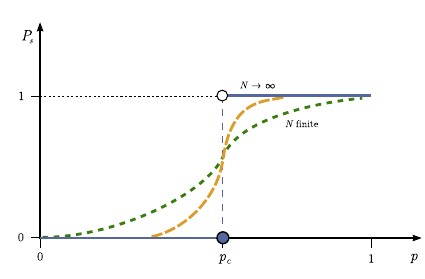
\includegraphics[width=\imsize]{probabilidad}
	\caption[Gráfico esquemático que ilustra la relación entre la probabilidad de percolación y la ocupación en un sistema]{Gráfico esquemático que ilustra la relación entre la probabilidad de percolación y la ocupación en un sistema. A medida que el tamaño del sistema ($N$) se aproxima a infinito, la probabilidad de percolación ($P_\infty$) converge hacia una función escalonada alrededor del umbral crítico ($p_c$). En determinados casos de sistemas altamente específicos, se observa una intersección en un punto único para todos los gráficos correspondientes a valores finitos de $N$. Sin embargo, debido a las correcciones de tamaño finito inherentes, en general esta intersección no ocurre en un único punto para sistemas finitos.}\label{fig:probabilidadinf}
\end{figure}

Es relevante destacar que, en general, los enlaces de una red tienen más vecinos cercanos que los sitios. Por lo tanto, los clústeres de enlaces se forman de manera más eficiente que los clústeres de sitios, lo que implica que se requiere una menor concentración de enlaces para generar un clúster expansivo. En otras palabras, el umbral de percolación de los enlaces es menor que el umbral de percolación de los sitios en una red dada \cite{bunde_fractals_2012}.



Dentro del campo de la percolación, un tema de investigación activo es la determinación precisa de los umbrales de percolación, ya sea mediante métodos exactos o simulaciones. Estos umbrales son una característica fundamental en la teoría de la percolación y su valor no es universal, sino que depende en gran medida de la estructura del grafo subyacente y su dimensionalidad. Se postula que los umbrales alcanzan valores de campo medio solo en el límite de dimensionalidad infinita \cite{Artem,fisher_cluster_2004}. Encontrar pruebas rigurosas de los umbrales y límites exactos ha sido un desafío constante para los investigadores \cite{kesten_critical_1980,wierman_bond_1984,grimmett_percolation_2013}. Aunque se han obtenido los umbrales exactos en 2D para redes cuadradas, triangulares, de panal y estructuras similares utilizando la transformación estrella-triángulo (ver \Cref{table:umbral}) \cite{wierman_bond_1984}, aún existen numerosos sistemas de interés para los cuales los umbrales exactos son desconocidos

 
 \begin{table}[h!]
 	\centering
 	\caption[Umbrales de percolación para varias redes en diferentes dimensiones y la red de Bethe. ]{ Umbrales de percolación para varias redes en diferentes dimensiones y la red de Bethe. La segunda columna enumera el número de vecinos más cercanos (nn), también conocido como número de coordinación. En una dimensión dada, se observa una disminución del umbral de percolación a medida que aumenta el número de vecinos más cercanos. La red o árbol de Bethe es una red no periódica infinita sin bucles cerrados (circuitos), en la cual cada sitio (excepto los múltiples sitios en la superficie) tiene un número de coordinación $Z$, que representa el número de enlaces conectados a dicho sitio.
 	}
 	\begin{tblr}{colspec={X[l,2]X[l,1]X[l,3]X[l,3]},
 			row{odd} = {bg=gray8},
 			row{even} = {bg=gray9},
 			row{1} = {bg=red3, fg=white, font=\sffamily},
 		}
 		
 		red	&  \# nn  &  {Percolación \\ de sitios}  &   {Percolación \\ de enlaces} \\
 		1d & $2$  & $1$ & $1$ \\
 		Triangular (2d) & $6$ &  $1/2$ & $2\sin(\pi/18)\approx 0.34729$ \\
 		Cuadrada (2d) &  $4$ &  $0.592746$ &  $1/2$ \\
 		Panal (2d)        &  $3$ &  $0.6962$ &  $1-2\sin(\pi/18)\approx0.65271$ \\
 		FCC (3d)           &  $12$ &  $0.198$   &  $0.119$ \\
 		BCC (3d)          &  $8$ & $0.246$    &  $0.1803$ \\ 
 		CS (3d) & $6$ &  $0.31161$ &  $0.248814$ \\
 		Diamante (3d) & $4$ & $0.43$ & $0.388$ \\
 		Hipercubo (4d) & $8$ & $0.197$ & $0.1601$ \\
 		Hipercubo (5d) & $10$ & $0.141$ & $0.1182$ \\
 		Hipercubo (6d) & $12$ & $0.107$ & $0.0942$ \\
 		Hipercubo (7d) &  $14$ & $0.089$ &  $0.0787$ \\
 		red de Bethe &  $z$ & $1/(z-1)$  &  $1/(z-1)$  \\
 	\end{tblr}
 	\label{table:umbral}
 \end{table}
 
 
 
 Consideremos un fragmento de la red cuadrada  $\mathbf{Z}^2$ como ejemplo ilustrativo de la definición anterior. En esta red, los puntos de intersección de las líneas se denominan \textquote{sitios}, mientras que los segmentos que los conectan se conocen como \textquote{enlaces}. En una red cuadrada, cada enlace se encuentra conectado a los seis enlaces vecinos más cercanos, mientras que cada sitio solo tiene cuatro sitios vecinos más cercanos. Se asume que cada sitio puede estar en uno de dos estados posibles: \textquote{vacío} o \textquote{abierto} (también se podría utilizar la terminología de \textquote{permitido}, aunque no existe una terminología universalmente aceptada para estos estados, y se podrían emplear términos como \textquote{encendido} o \textquote{apagado}). Además, se considera que la apertura de un sitio ocurre de manera aleatoria e independiente de sus vecinos, con una probabilidad $p$. En esta red, cada par de sitios vecinos más cercanos está conectado por un enlace. Cuando se observa que un poco más de la mitad de los sitios están abiertos (\Cref{fig:percolacion_enlaces_sitios}b, centro), se evidencia una tendencia de los sitios abiertos a agruparse en clústeres de diversas formas y tamaños. Estos clústeres pueden ser clasificados de acuerdo a su tamaño. Por ejemplo, un grupo de tamaño $1$ corresponde a un solo sitio abierto sin vecinos abiertos inmediatos, mientras que un grupo de tamaño $2$ consiste en dos sitios abiertos adyacentes sin vecinos abiertos, y así sucesivamente.
 
 
 
 Cuando la probabilidad $p$ se incrementa a $0.605$ (\Cref{fig:percolacion_enlaces_sitios}b, derecha), se observan varios fenómenos significativos. 
 En primer lugar, con una probabilidad entre $1/2$ y $2/3$, muchos de los sitios se unen en un \textquote{clúster gigante} que abarca tanto la matriz en sentido vertical como horizontal . Esta probabilidad crítica $p_c$, es aproximadamente $p_c \approx 0.593$  para los sitios de la red cuadrada. Un enfoque analógico se puede realizar considerando un \textquote{fluido} que únicamente puede fluir a través de los enlaces que conectan sitios abiertos. Por debajo del umbral de la probabilidad crítica, la red presenta una conductividad cero, mientras que por encima de dicho umbral, la conductividad aumenta a medida que se incrementa la probabilidad. De esta manera, se establece una fuerte relación entre la conectividad de los elementos microscópicos del sistema y las propiedades físicas a nivel macroscópico. Además, a medida que se incrementa la proporción de sitios abiertos, también aumenta la proporción de sitios vacíos con vecinos abiertos. Este aumento en la proporción de sitios vacíos conectados a vecinos abiertos tiene implicaciones significativas en el comportamiento global del sistema.
 
  

\begin{figure}[h!]
	\centering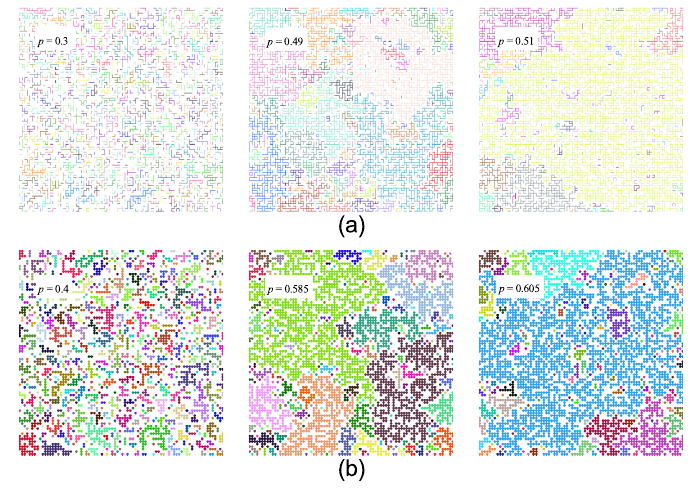
\includegraphics[width=\imsize]{percolacion_enlaces_sitios.png}
	\caption[Diagramas esquemáticos que ilustran la percolación clásica en una red cuadrada.]{Diagramas esquemáticos que ilustran la percolación clásica en una red cuadrada. En estos diagramas, se utilizan diferentes colores para representar clústeres distintos. El tamaño del sistema utilizado es $N = L \times L = 80 \times 80$. Los valores de $p$ etiquetados en las figuras corresponden a las probabilidades de ocupación de los sitios o enlaces correspondientes. (a), se muestra la percolación de enlaces, donde se omiten los sitios y enlaces no ocupados para facilitar la identificación. Para un valor de $p = 0.51$, se observa la existencia de un clúster gigante destacado en color amarillo.(b), se ilustra la percolación de sitios, nuevamente omitiendo los enlaces y sitios no ocupados para una mejor visualización. Para $p = 0.605$, se identifica un clúster gigante en color azul (adaptado de \protect\cite{li_percolation_2021}).}\label{fig:percolacion_enlaces_sitios}
\end{figure}


Una vez que se supera el umbral crítico $p_c$, se observa que el flujo de fluido en la red ocurre exclusivamente a través de los enlaces que conectan los sitios abiertos. Al examinar la estructura resultante, se evidencia la presencia de una columna vertebral compuesta por enlaces que permiten el flujo continuo del fluido, mientras que otros enlaces se convierten en callejones sin salida aislados o ramas colgantes. La proporción de estas ramas varía en función del valor de $p$. La función de accesibilidad se define como la proporción de sitios abiertos que forman parte del clúster infinito, es decir, aquellos que serían atravesados por el fluido en los límites de la red.  A medida que incrementa el valor de $p$, los clústeres experimentan un crecimiento y se fusionan entre sí, mientras que los sitios vacíos se fragmentan y se agrupan en clústeres más pequeños. Cabe destacar que el ejemplo mencionado anteriormente corresponde a la percolación de sitios, donde se varía exclusivamente la proporción de sitios abiertos. Existe también un procedimiento similar conocido como percolación de enlaces, en el cual se varía la proporción de enlaces abiertos (\Cref{fig:percolacion_enlaces_sitios}a). Es importante tener en cuenta que estos dos procedimientos no son intercambiables y no existe una fórmula simple que permita predecir la percolación de enlaces a partir de la percolación de sitios. Además, el valor crítico $p_c$ para la percolación de sitios siempre es mayor que el valor crítico $p_c$ para la percolación de enlaces (consultar \Cref{table:umbral}).


El contorno irregular y \textquote{ramificado} de un clúster en percolación presenta similitudes con los fractales. De hecho, se ha demostrado que los clústeres cercanos al umbral de percolación exhiben propiedades fractales \cite{aharony_introduction_2017}. La dimensión fractal de un clúster de percolación es aproximadamente constante ($D \approx 1.896$) independientemente del tipo de red bidimensional utilizada, ya sea cuadrada, triangular, de panal, de Voronoi u otra (\Cref{fig:distitnasredes}a–d), a pesar de las diferencias en sus conectividades, las cuales pueden ser cuantificadas mediante el número de coordinación $z$, definido como el promedio de enlaces por sitio. No obstante, la dimensión fractal varía según la dimensionalidad o la dimensión de incrustación $d$ de la red. Por ejemplo, los clústeres que se percolan en redes bidimensionales presentan dimensiones fractales distintas a las de las redes tridimensionales, como las redes cúbicas (\Cref{fig:distitnasredes}e).



\begin{figure}[h!]
	\centering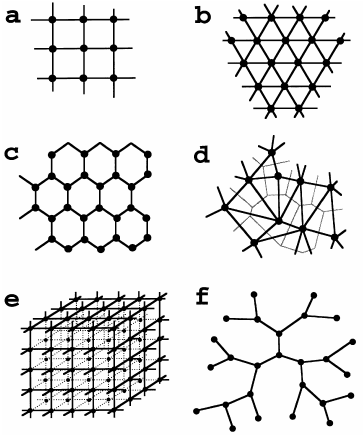
\includegraphics[width=\imsize]{distitnasredes.png}
	\caption[Ejemplos de redes bidimensionales.]{ Ejemplos de redes bidimensionales, en las cuales los sitios son representados por círculos, mientras que los enlaces se muestran mediante líneas oscuras. En esta figura, se exhiben diversas configuraciones de redes: (a) una red cuadrada con  $z=4$, (b) una red triangular con  $z=6$, (c) una red tipo panal con $z=3$, (d) una red Voronoi con un grado promedio de conectividad de $\left\langle z \right\rangle = 6$, (e) una red cúbica con  $z=6$, y (f) un árbol de Cayley con  $z=3$ (adaptado de \protect\cite{berkowitz_percolation_1998})}\label{fig:distitnasredes}
\end{figure}






\section{Fundamentos matemáticos de la percolación}\label{sec:matematicaspercolacion}

Se considera un grafo $G=(V,E)$, donde $V$ representa el conjunto de vértices y $E$ el conjunto de aristas. En el marco del modelo de percolación de enlace, cada arista tiene la capacidad de abrirse de manera independiente con una probabilidad $p$ o cerrarse con una probabilidad $1-p$. Este fenómeno se describe mediante la medida de probabilidad $P_p$. El conjunto de aristas abiertas forma así un subgrafo aleatorio de $G$ y la pregunta original formulada por Broadbent se centra en determinar si la componente conexa del origen en este subgrafo aleatorio es finita o infinita \cite{beffara_percolation_2006}.



Se define un camino en $G$ como una secuencia $v_1, v_2, \cdots$ en la cual cada par de vértices sucesivos, $v_i$ y $v_{i +1}$, se encuentran conectados mediante una arista en $G$. Un camino se considera abierto si todas las aristas $\left\{v_i,v_{i+1}\right\}$ que lo componen están en estado abierto. El clúster infinito del origen se refiere a la existencia de un camino abierto ilimitado que se origina en el vértice de origen. Además, se presenta un modelo análogo denominado percolación del sitio, en el cual todas las aristas son transitables, aunque cada vértice puede encontrarse en estado abierto o cerrado de manera independiente, con probabilidades $p$ y $1 - p$, respectivamente. En este caso, se define un camino abierto como aquel en el cual todos los vértices a lo largo del camino se encuentran en estado abierto.

 Se asume que todos los grafos considerados son conexos, localmente finitos y cuasi-transitivos. Si $A$ y $B$ son subconjuntos de vértices en $V$, se establece que $A\leftrightarrow B$ si existe un camino abierto que conecta algún vértice en $A$ con algún vértice en $B$. Para simplificar la notación, se utiliza la notación $u \leftrightarrow v$ para denotar la existencia de un camino entre los vértices $u$ y $v$, es decir, el evento $\left\{u\right\} \leftrightarrow \left\{v\right\}$. El clúster abierto $C(v)$  de un vértice $v$ se define como el conjunto de todos los vértices abiertos que se encuentran conectados a $v$ mediante un camino abierto:

\begin{equation}\label{eq:1}
	C(v) = \left\{u\in V: u \leftrightarrow v \right\}
\end{equation}

La probabilidad de percolación $\theta(p)$  se considera el parámetro central en la teoría de la percolación, y representa la probabilidad de que un sitio seleccionado aleatoriamente pertenezca a un clúster infinito \cite{torquato_percolation_2002}. Es importante resaltar que $\theta(p)$  siempre es menor que $p$, excepto en el caso trivial cuando $\theta(p) = p = 1$. En un sistema infinito, la probabilidad de percolación es cero para valores de $p$ por debajo de $p_c$.


\begin{equation}\label{eq:2}
\theta(p)  \coloneqq P_\infty = P_p\left\{\mathbf{0} \leftrightarrow \infty\right\} = P_p\left\{\left| C(\mathbf{0})\right|=\infty \right\}  = \begin{cases}
	0 & \text{sí } p<p_c\\
	>0 & \text{sí } p>p_c
\end{cases}
\end{equation}

El modelo de percolación se distingue por su propiedad más destacada: la presencia de una transición de fase geométrica, en la cual el parámetro $\theta(p)$ desempeña el papel de un parámetro de orden en una transición de fase termodinámica. Esta transición se produce en un valor crítico $p_c \in  [0 , 1]$, donde el comportamiento global del sistema experimenta cambios sustanciales en dos regiones distintas: $p < p_c$ y $p > p_c$.  Para definir esta propiedad de forma rigurosa, se emplea la construcción conjunta de sistemas de percolación de Hammersley \cite{broadbent_percolation_1957}  en el grafo $G$. Se considera una colección de variables aleatorias independientes $\left\{U(v),v\in V\right\}$, distribuidas uniformemente en el intervalo $[0,1]$. Un vértice $v$ se declara como $p$-abierto si $U(v) \leq p$; de lo contrario, se declara como $p$-cerrado. La configuración de vértices $p$-abiertos sigue la distribución $P_p$ para cada valor de $p\in [0, 1]$. Es relevante destacar que la colección de vértices $p$-abiertos no disminuye a medida que $p$ aumenta, lo que implica que $\theta(p)$ también es una función no decreciente. Esta propiedad se puede demostrar observando que $\theta(0) = 0$ y $\theta(1) = 1$  (ver \Cref{fig:probabilidadtheta}). Por lo tanto, $\theta(p)$  juega un papel fundamental como parámetro de orden en la transición de fase.



\begin{figure}[h!]
	\centering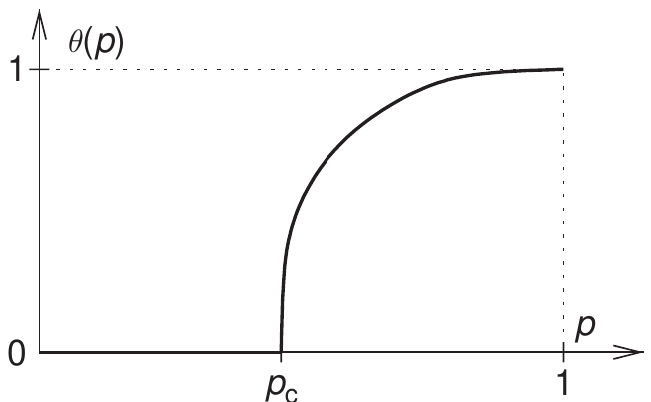
\includegraphics[width=\imsize]{probabilidadtheta.png}
	\caption[El comportamiento de la función $\theta(p)$ en las cercanías del punto crítico.]{El comportamiento de la función $\theta(p)$ en las cercanías del punto crítico.}\label{fig:probabilidadtheta}
\end{figure}


El valor crítico o umbral de percolación $p_c$ se define formalmente (para un sistema infinito) como:

\begin{equation}\label{eq:3}
p_c \coloneqq p_c( G) = \sup\left\{p:\theta(p)=0\right\},
\end{equation}


donde $\sup$ representa el supremo, es decir, el límite superior mínimo. Cuando $p < p_c$, el clúster abierto que contiene el origen es finito, lo que implica que todos los clústeres también son finitos. En contraste, cuando $p > p_c$, la distribución $P_p$ presenta una probabilidad estrictamente positiva de que el clúster que contiene el origen sea infinito. Por lo tanto, $p_c$ marca la transición en la cual el comportamiento global del sistema experimenta un cambio significativo.



\begin{theorem}[Ley Cero-Uno de Kolmogórov] % Specify a name/title in square brackets, or leave them out for no title
	Sea $\omega(e)_e$  una secuencia de variables aleatorias independientes e idénticamente distribuidas, y $A$ un evento de cola. Entonces, se cumple que $\mathbb{P}[A] \in {0, 1}$ .
\end{theorem}

La Ley Cero-Uno de Kolmogórov establece que 

\begin{equation}\label{eq:4}
P_p\left\{\left| C(v)\right| =\infty \ \text{para algún} \ v \in  V  \right\} = 1 \ \text{para} \quad p>p_c
\end{equation}

Esta ley implica que cuando el valor de $p$ supera el umbral $p_c$, se garantiza que al menos un vértice $v \in V$ pertenezca a un clúster de tamaño infinito.
Por lo tanto, si los intervalos $[0, p_c)$ y $(p_c, 1]$ no están vacíos, se produce una transición de fase en $p_c$. Esta transición de fase indica un cambio cualitativo en el comportamiento del sistema al cruzar el umbral $p_c$.  Utilizando el argumento de Peierls, es posible demostrar de manera sencilla que $p_c(G )$ es mayor que cero para cualquier grafo $G$ con un grado acotado. Este resultado implica que en todos los grafos $G$  con grados acotados, se establece un valor umbral $p_c$ por encima del cual el sistema exhibe una fase supercrítica, donde es probable la existencia de clústeres de tamaño infinito.


\section{La percolación como fenómeno crítico}\label{sec:percolacion_critico}


En la sección anterior, se exploró la percolación como una transición de fase geométrica  que ocurre cuando la concentración crítica $p_c$ divide el sistema en dos fases distintas: una con clústeres finitos ($p < p_c$) y otra con un clúster de gran tamaño ($p > p_c$). Es importante destacar que una verdadera transición de fase se presenta únicamente en sistemas infinitos, conocidos como el \textquote{límite termodinámico}. En este contexto, la concentración crítica $p_c$ se define de forma única en sistemas infinitos. La transición de percolación se caracteriza por las propiedades geométricas de los clústeres cercanos a $p_c$. Un parámetro clave en este sentido es la probabilidad $P_\infty$, definida mediante la  \cref{eq:2}. Esta probabilidad es nula por debajo de $p_c$ y distinta de cero por encima de $p_c$. Para valores ligeramente superiores a $p_c$, se establece una relación de la forma

 \begin{equation}\label{eq:10}
	P_\infty \propto \left(p-p_c\right)^\beta,
\end{equation}

donde $\beta$ es el \textquote{exponente crítico}. El comportamiento crítico en la teoría de la percolación se refiere al estudio de la red infinita y los clústeres grandes pero finitos en las cercanías de $p_c$, también conocido como región de escalamiento. En esta región, se observa un comportamiento crítico independiente de las propiedades locales del sistema, como el tipo de red y el mecanismo de percolación. Esto se debe al principio de universalidad, que establece que el valor de $p_c$ está determinado por la estructura local del sistema, mientras que el comportamiento de los clústeres cercanos a $p_c$ es independiente de dicha estructura local. En consecuencia, la percolación se considera un fenómeno dependiente del sustrato pero independiente del modelo específico. Los exponentes críticos, como $\beta$, son determinados exclusivamente por la geometría del sistema y son idénticos tanto en la percolación de enlaces como en la percolación de sitios.

 \subsection{Parámetro de orden}\label{sec:parametro_orden}
 
 
 
 
 
La teoría de escalamiento de los clústeres de percolación es el enfoque más elegante para caracterizar la percolación como un fenómeno crítico \cite{stauffer_scaling_1979}. En términos de estadísticas de clústeres, se puede formular gran parte de la teoría de la percolación, lo que facilita establecer analogías con otras transiciones de fase. En este sentido, se propone la definición de un parámetro de orden que permita caracterizar nuestro modelo de criticidad neuronal a través de observables geométricos. En el contexto de la percolación, los clústeres desempeñan un papel fundamental.
 
 
\begin{definition}[clúster] % Specify a name/title in square brackets, or leave them out for no title
Un clúster se define como  un conjunto de componentes o elementos interconectados en una red, donde la conexión entre ellos se establece mediante vínculos o relaciones específicas.
\end{definition}

Se consideran clústeres de tamaño unitario a los nodos aislados, mientras que se denomina $s$-clúster a cualquier conjunto de $s$ nodos conectados. El análisis de la percolación se centra en la aparición del clúster infinito a medida que aumenta la probabilidad $p$. Una medida común para caracterizar este fenómeno es la probabilidad $\bar{S}_1/N$ de que un nodo pertenezca al clúster infinito, donde $N$ representa el tamaño del sistema (número de sitios) y $\bar{S}_1$ es el promedio en ensamble del número de sitios $S_1$ en el clúster más grande.  Como se ilustra en la \cref{fig:probabilidadtheta}, a medida que $p$ aumenta, también lo hace la probabilidad de encontrar clústeres de mayor tamaño. En una red finita, como se muestra en la \cref{fig:percolacion_enlaces_sitios}, se identifica un valor crítico $p_c$ por encima del cual al menos un clúster conecta los extremos \textquote{inferior} y \textquote{superior} (o \textquote{izquierdo} y \textquote{derecho}) de la red. En otras palabras, se establece un punto crítico $p_c$ para el cual $\bar{S}_1/N$ adquiere un valor distinto de cero. En el campo de la ciencia de redes, el tamaño del clúster más grande se considera un parámetro de orden preferido. En el umbral de percolación, este parámetro de orden muestra un comportamiento crítico a medida que el sistema tiende al límite $N \to\infty$. Dicha relación puede expresarse de la siguiente manera:

\begin{equation}\label{eq:5}
	P_\infty = \lim_{N\to\infty} \frac{\bar{S}_1}{N} =  \begin{cases}
		0 & \text{sí } p<p_c\\
		a\left(p-p_c\right)^\beta & \text{sí } p>p_c
	\end{cases}
\end{equation}

donde $a$ representa una constante y $\beta$ es el exponente crítico del parámetro de orden. La formulación basada en la teoría de escalamiento de los clústeres de percolación permite una caracterización precisa de la transición de fase en el modelo de criticidad neuronal abordado en esta parte de la tesis. Al introducir un parámetro de orden, se establece una conexión rigurosa entre las propiedades estadísticas de los clústeres y la dinámica coordinada de la actividad neuronal en el organismo modelo C. elegans. 


\subsection{ El tamaño promedio de los clústeres  $ \chi(p)$}\label{sec:Sucebtibilidad}

Como la percolación es un proceso estocástico se da lugar a la formación de clústeres con una amplia variedad de tamaños y formas en diversas redes \cite{aharony_introduction_2017}. Para analizar las propiedades estadísticas promedio de estos clústeres, es necesario examinar sus distribuciones. En particular, se investiga la distribución del tamaño de los clúster  \( p_s=\frac{m_s}{\sum_{s}m_s} \), donde $m_s$ representa el número de clústeres de tamaño $s$ presentes en una red de tamaño $N$. Además, se utiliza comúnmente la distribución normalizada de tamaño de clústeres, \(n_s=\frac{m_s}{N}\), que indica la cantidad de clústeres de tamaño $s$ por nodo en la red, considerando la probabilidad de percolación $p$ \cite{barrat_dynamical_2008}. La probabilidad de que un nodo $i$ pertenezca a un clúster de tamaño $s$ se denota como $sn_s(p)$, donde $i$ puede ser cualquier elemento del clúster en cuestión. Es importante destacar que \(p_s=\frac{n_sN}{\sum_{s}m_s}=n_s\left\langle S \right\rangle \), donde \(\left\langle S \right\rangle =\frac{N}{\sum_{s}m_s} = \sum_{s} sP_s \) representa el tamaño promedio del clúster. Cabe señalar que el tamaño promedio \(\left\langle  S \right\rangle \)   difiere del tamaño promedio de clúster \(\chi\) , el cual se define más adelante. La probabilidad $p$ de que un sitio esté ocupado se puede expresar como la suma de estas probabilidades para todos los tamaños posibles. En el caso de $p < p_c$, esta relación se formula de la siguiente manera:

\begin{equation}\label{eq:12}
p=\sum_{s}{sn_s}(p)
\end{equation}

Cuando $p > p_c$, se observa la presencia de un clúster gigante, en el cual cada nodo tiene una probabilidad finita $\bar{S}_1/N > 0$ de formar parte del mismo. Por otro lado, los demás clústeres presentan un tamaño finito $s$ para cualquier valor arbitrario de $p$, y su comportamiento se describe mediante la distribución de tamaño de clúster $n_s(p)$. Por lo tanto, la suma de todas las probabilidades de que un nodo dado pertenezca a un clúster de tamaño finito, excluyendo el clúster gigante, debe ser igual a $p$:

\begin{equation}\label{eq:13}
	p=P_\infty+{\sum_{s}}^{\prime}sn_s(p) 
\end{equation}

Aquí, la suma ${\sum_{s}}^{\prime}$ abarca todos los valores finitos de $s$, lo cual implica que el clúster gigante se excluye de dicha suma. Resulta primordial establecer una medida objetiva para cuantificar con precisión el tamaño de los clústeres.  Al analizar el fenómeno de la percolación, se observa de manera intuitiva que, a medida que el valor de $p$ disminuye, el tamaño de los clústeres es pequeño, mientras que su tamaño tiende a aumentar a medida que $p$ se incrementa, hasta llegar a un umbral crítico donde el clúster gigante adquiere un rol dominante, por lo que el tamaño de los clústeres debe divergir \cite{saberi_recent_2015}. No obstante, una vez superado dicho umbral, es imperativo excluir al clúster gigante de los análisis, ya que su presencia constante puede sesgar los resultados. Además, a medida que los clústeres son absorbidos por el clúster gigante, el tamaño promedio de los clústeres restantes vuelve a disminuir. Por consiguiente, buscamos una medida que exhiba un comportamiento creciente, divergente en el umbral crítico y, posteriormente, decreciente (véase la \Cref{fig:promedio}). Aplicando el teorema de Bayes, podemos expresar de forma rigurosa la probabilidad condicional de que un nodo ocupado pertenezca a un clúster de tamaño $s$ mediante la siguiente formulación:

\begin{equation}\label{eq:14}
w_s(p) = \frac{sn_s(p)}{{\sum_{s}}^{\prime}sn_s(p)}
\end{equation}

Con base en esto, definimos el tamaño promedio de los clústeres $\chi(p)$  a los cuales pertenece cualquier nodo ocupado como:

\begin{equation}\label{eq:15}
\chi(p)={\sum_{s}}^{\prime}{sw_s(p)}=\frac{{\sum_{s}}^{\prime}{s^2n_s(p)}}{{\sum_{s}}^{\prime}{sn_s(p)}}
\end{equation}

Es importante resaltar que, al considerar las sumas ${\sum_{s}}^{\prime}$, no se toma en cuenta la divergencia generada por la presencia del clúster gigante. Sin embargo, la definición proporcionada por la \cref{eq:15} carece de información sobre la estructura de los clústeres, como su compacidad y extensión espacial. No obstante, resulta imprescindible abordar esta limitación y analizar la extensión geométrica de los clústeres. Para tal propósito, se consideran los sitios pertenecientes a un clúster de tamaño $s$, representados por las coordenadas $\mathbf{r}_i$, donde $i = 1, 2,\cdots,s$. Con el fin de examinar de manera más exhaustiva la estructura interna, se introduce el concepto de centro de masa del clúster, $\mathbf{r}_0 = \sum{\mathbf{r}_i}/s$, definido como el promedio de las coordenadas de los sitios, dividido por el tamaño del clúster $s$. A partir de esta definición, se plantea el concepto de radio de giro del clúster, $R_s$, que se obtiene al calcular la raíz cuadrada de la suma de las distancias al cuadrado entre cada sitio y el centro de masa, dividida por el tamaño del clúster $s$:

\begin{equation}\label{eq:19}
R_s^2=	\frac{\sum{\left(\left| \mathbf{r}_i-\mathbf{r}_0\right|^2 \right)}}{s}=\frac{1}{2s^2}\sum_{i,j}{\left|\mathbf{r}_i-\mathbf{r}_j\right|^2}
\end{equation}

Este parámetro permite evaluar la distancia promedio entre dos sitios dentro del mismo clúster. Un valor menor de $R_s$ indica una mayor compacidad y una menor extensión espacial del clúster en cuestión. Adicionalmente, otro aspecto relevante para describir la estructura de los clústeres es la longitud de correlación, $\xi$. Esta medida se basa en la función de correlación de dos puntos, $g_c(r )$, que representa la probabilidad de que dos puntos se encuentren en el mismo clúster, dada una distancia $r$ entre ellos. Por lo general, esta función sigue un patrón de decaimiento exponencial expresado como:


\begin{equation}\label{eq:16}
g_c(r) \sim e^{-r/\xi},  \ r\to\infty
\end{equation}

La longitud de correlación, $\xi$, constituye una escala característica de la distribución de clústeres y establece la distancia máxima a partir de la cual los clústeres se vuelven escasos de manera exponencial. Además, $\xi$ delimita la región de escala en la cual los clústeres de percolación exhiben un comportamiento autosimilar. Para calcular $\xi$, se utiliza la siguiente relación:

\begin{equation}\label{eq:17}
\xi^2=\frac{\sum_r{r^2g_c(r)}}{\sum_r{g_c(r)}}
\end{equation}

Dentro de esta expresión, se reemplaza $r^2$  en la suma anterior por el cuadrado de la distancia promedio entre dos puntos del clúster, es decir, $2R_{s}^2$. Asimismo, considerando la probabilidad $sn_s$ de que un punto pertenezca a un clúster de tamaño $s$ y teniendo en cuenta que dicho punto está conectado a $s$ sitios, se sustituye $g_c(r)$ por $s^2n_s$. Esto nos lleva a la siguiente relación para el cuadrado de la longitud de correlación:

\begin{equation}\label{eq:18}
	\xi^2(p)=\frac{{\sum_s}^{\prime}{2R_{s}^2s^2n_s(p)}}{{\sum_{s}}^{\prime}{s^2n_s(p)}}
\end{equation}

Estas definiciones de los diferentes parámetros característicos son aplicables en todas las dimensiones $d$.



\begin{figure}[h!]
	\centering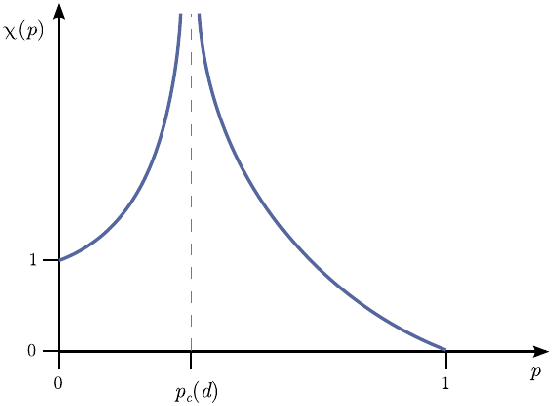
\includegraphics[width=\imsize]{promedio.png}
	\caption[Evolución del tamaño promedio de los clústeres finitos y la longitud de correlación cerca de la transición percolativa.]{ Evolución del tamaño promedio de los clústeres finitos y la longitud de correlación cerca de la transición percolativa. Como se puede observar en el diagrama, al alcanzar el umbral crítico $p_c$, se evidencia la aparición del componente gigante, lo que implica la presencia de clústeres de distintos tamaños en el sistema en estudio. Asimismo, se aprecia que la longitud de correlación experimenta un aumento significativo, indicando una relación proporcional con el tamaño del sistema $L$.}\label{fig:promedio}
\end{figure}


\subsection{Teoría de escala y exponentes críticos}



El comportamiento del proceso de percolación en un sistema está estrechamente ligado a su posición en el régimen subcrítico ($p < p_c$) o supercrítico ($p > p_c$). En el régimen subcrítico, la probabilidad de encontrar un clúster finito $s$ de gran tamaño en un punto dado disminuye exponencialmente con $s$, lo que implica una distribución de tamaños de clúster con una cola de decaimiento exponencial. Esta disminución exponencial puede ser descrita mediante el parámetro $\kappa(p) > 0$, que $\kappa(p) \to\infty$ cuando $p\to0$, y $\kappa(p = p_c ) = 0$. En otras palabras, se puede aproximar la distribución de tamaños de clústeres utilizando la expresión:

\begin{equation}\label{eq:20}
w_s(p) \approx e^{-\kappa(p)s}, \ s\to\infty
\end{equation}

Por otro lado, en el régimen supercrítico, la cola de la distribución de tamaños de clústeres finitos muestra un decaimiento más suave. En este caso, existen dos funciones,  $\kappa_1(p)$  y $\kappa_2 (p)$, que cumplen con $0 < \kappa_2(p) \leq  \kappa_1(p) < \infty$ \cite{grimmett_percolation_2013}, tales que:

\begin{equation}\label{eq:21}
	\exp{\left(-\kappa_1(p)s^{\frac{d-1}{d}}\right)} \leq w_s(p) \leq \exp{\left(-\kappa_2(p)s^{\frac{d-1}{d}}\right)}
\end{equation}

Además, la potencia $s^{(d-1)/d}$, que representa el orden del área superficial de una esfera en $d$ dimensiones con volumen $s$, indica que los clústeres son compactos en la región supercrítica \cite{djordjevic_scaling_1987}. Es importante destacar que, aunque el valor numérico de las cantidades que caracterizan la percolación depende de los detalles microscópicos del sistema, como el número de conexiones entre los nodos, cerca del umbral de percolación $p_c$, la mayoría de estas cantidades siguen leyes de escala que son ampliamente independientes de la estructura de la red y sus detalles microscópicos. En consonancia con la hipótesis de escala, se establece una relación general entre el número $n_s(p)$ de clústeres finitos por sitio y el tamaño $s$, dada por:
\begin{equation}\label{eq:22}
	n_s(p)  \propto s^{-\tau}F\left(c(p)s\right), \ s\to\infty,
\end{equation}

Donde $\tau$ es un exponente libre y $F$ es una función de escala.  Además, cerca del umbral de percolación, se ha observado que  $c(p)$ puede ser descripta mediante una ley de potencia general, $c (p) \propto \left|p-p_c \right|^{1/\sigma}$, donde $\sigma$ es otro exponente crítico.  En relación con la distribución del tamaño de los clústeres, se pueden considerar los $m$-ésimos momentos, definidos como $M_m(p) = \sum_{s}s^mn_s(p)$, con $m \geq 1$. También se ha conjeturado la existencia de relaciones de escala cerca del umbral de percolación que involucran diferentes exponentes críticos, tales como $\beta$, $\gamma$, $\alpha$, $\Delta$,  $\tau$ y $\nu$:


\begin{align} 
	P_\infty(p) & \simeq B\left(p-p_c\right)^\beta, \label{eq:6a}\\ 
	\chi(p)  & \simeq \Gamma^{\pm}\left| p-p_c \right|^{-\gamma}, \label{eq:6b} \\
	n_s(p) & \simeq A^{\pm}  \left| p-p_c \right|^{2-\alpha}, \label{eq:6c} \\
	\frac{M_{m+1}(p)}{M_m(p)} &\simeq D^{\pm} \left| p-p_c \right|^{-\Delta}, \label{eq:6d}\\
	\xi(p) &\simeq f^{\pm}\left| p-p_c \right|^{-\nu}, \label{eq:6e} \\
	s_\xi(p) &\simeq \left| p-p_c \right|^{-\frac{1}{\sigma}}, \label{eq:6f}\\
	p_s &\propto s^{-\tau}.
	\end{align}
	
	
que también definen las amplitudes críticas, donde estas desempeñan un papel crucial al determinar las magnitudes que se acercan al punto crítico ($p_c$), ya sea desde arriba o desde abajo, indicadas por los superíndices $+$ o $-$. Estas amplitudes combinadas proporcionan una forma canónica de codificar la información universal relacionada con la aproximación a la criticidad \cite{aharony_universal_1980}. La caracterización del comportamiento crítico de la transición de percolación se basa en los exponentes  $\beta$, $\gamma$, $\alpha$, $\Delta$,  $\tau$ y $\nu$. Estos exponentes, conocidos como exponentes críticos, describen las propiedades geométricas de la transición y son independientes de los detalles estructurales de la red, como su forma (cuadrada o triangular), así como del tipo de percolación (sitio, enlace o continua). En cambio, su valor depende únicamente de la dimensión $d$ de la red.  La propiedad de universalidad, inherente a las transiciones de fase en general, también se manifiesta en la transición de percolación. En esta transición, el parámetro de orden experimenta una desaparición continua en el punto crítico. Esto se refleja en el comportamiento característico de ley de potencia y funciones singulares observado en el umbral de percolación. Estos fenómenos indican que el sistema exhibe grandes fluctuaciones en sus propiedades estadísticas antes de la aparición de una fase macroscópicamente ordenada, como la formación de una estructura global conexa. Cuando las fluctuaciones alcanzan el tamaño del sistema en el punto crítico, el sistema experimenta una transición hacia una nueva fase con orden macroscópico \cite{barrat_dynamical_2008}.

	
Es importante destacar que todas las cantidades mencionadas se definen en el límite termodinámico de sistemas de gran tamaño \cite{bunde_fractals_2012}. Sin embargo, hasta el momento, no se ha logrado obtener cálculos exactos y rigurosos de los exponentes críticos para la percolación, ni siquiera para otras transiciones de fase \cite{stauffer_scaling_1979}. El objetivo de una teoría de escala, en este contexto, es establecer relaciones entre estos exponentes críticos. Dicha teoría se basa en un enfoque fenomenológico que se limita a relacionar magnitudes medibles sin requerir el cálculo directo de las mismas. Asimismo, es importante tener presente que los exponentes no son independientes entre sí, sino que satisfacen las relaciones de escala expresadas por:


 \begin{align}\label{eq:7}
 	&\beta = \Delta\left(\tau-2\right)=\frac{\tau-2}{\sigma},\\
 	&\gamma=\frac{3-\tau}{\sigma},\\
 	&2-\alpha= \gamma + 2\beta =\frac{\tau-1}{\sigma}.\\	
 	 \end{align}



\subsection{ Teoría de  escala en el número de clústeres }\label{sec:num_clusteres}


Se pretende determinar el comportamiento asintótico del número de clústeres en el umbral, $n_s(p_c)$.  Se ha observado una relación proporcional entre el tamaño de los clústeres y su segundo momento, expresada como  $\chi \propto \sum_s s^2n_s$,   la cual se mantiene constante en el umbral debido a un denominador finito.  
Sin embargo, cuando $p = p_c$, esta suma se vuelve infinita, mientras que para cualquier otro valor de $p$ permanece finita. Se postula que un decaimiento de ley de potencia es más plausible para el número de clústeres $n_s(p_c)$, lo cual implica que el tamaño promedio de los clústeres, $\chi$, seguiría siendo finito en $p = p_c$. Por lo tanto, se define el exponente $\tau$ de Fisher (modelo de gotas de Fisher \cite{fisher_theory_1967}) mediante la relación $n_s(p_c) \propto s^{-\tau}$, considerando valores grandes de $s$. Con el fin de minimizar los errores en los cálculos numéricos, es común calcular la función de distribución acumulada complementaria (CCDF) de la distribución de tamaños de clústeres, que representa la probabilidad de que los clústeres tengan un tamaño mayor que $s$,

\begin{equation}\label{eq:36}
CCDF=P_{acc}(s)=\int_{0}^{\infty}n_sd_s=\int_{0}^{\infty}{s^{-\tau}}ds\propto s^{1-\tau}
\end{equation}
En este contexto, la distribución de clústeres sigue una relación de escala:


\begin{equation}\label{eq:37}
n_s\sim s^{1-\tau}f\left(\frac{s}{s^{*}}\right) \ \text{donde} \ s^*=\left| p_c-p\right|^{-\frac{1}{\sigma}}
\end{equation}

Es importante destacar que, en el caso de redes con tamaño finito $N < \infty$, la distribución de clústeres sigue una relación de escala modificada expresada como:

\begin{equation}\label{eq:38}
P(s)\sim s^{1-\tau}g\left(\frac{s}{s^\prime}\right) \ \text{donde} \ s^{\prime} \sim \xi^{d^c_f}
\end{equation}

Además, al asumir que $\xi\sim L$, podemos inferir que

\begin{equation}\label{eq:39}
s^{\prime} \sim L^{d_f^c}\sim N^{\frac{d_f^c}{d}}
\end{equation}

En las redes con tamaño $N < \infty$, el valor de $s^{\prime}$ es proporcional al tamaño del segundo clúster más grande ($S_2$) en la red ($S_2 \propto  s^{\prime}$). Por lo tanto, para derivar la dimensión fractal, se utiliza el valor de $S_2$, lo cual resulta útil para analizar la estructura de los clústeres en la red y obtener información relevante \cite{tesis_Mahdi}.



\subsection{Estructura fractal de los clústeres en el fenómeno de percolación}

La teoría de la escala postula que el comportamiento de un sistema, cuando se analiza a escalas de longitud inferiores a la longitud de correlación $\xi$, se asemeja al estado umbral. En el punto crítico, donde $\xi$ representa la única escala de longitud que determina el comportamiento crítico de una red infinita, la longitud de correlación tiende a infinito ($\xi\to\infty$). Esta desaparición de escala en $p = p_c$ evoca la invariancia de escala, la cual implica la aparición de autosimilitud en las características geométricas de los clústeres de percolación. En el contexto de los clústeres de percolación, las propiedades fractales persisten incluso cuando $p = p_c$ y $\xi$ es finita, siempre y cuando la escala de longitud utilizada para el estudio del sistema sea menor que $\xi$. Sin embargo, una vez que se supera la longitud de correlación, la geometría adquiere una forma euclidiana. Para una comprensión más precisa de este fenómeno, se considera un sistema de percolación observado a través de una ventana hipercúbica de tamaño $L^d$, donde $L$ representa el tamaño lineal de la ventana o puede interpretarse como el tamaño de un sistema finito.

Dentro del marco teórico de la invariancia de escala, se deduce que la masa media $M$ de los clústeres dentro de la ventana aumenta siguiendo una ley de potencias en relación con el tamaño, es decir, $M(\xi,L)\sim L^{d_f^c}$, donde $d_f^c$ representa la dimensión fractal del clúster. Esta dimensión fractal describe cómo, en promedio, la masa $M$ del clúster dentro de una esfera de radio $r $ escala con $r$:

\begin{equation}
	M(r)\sim r^{d_f^c}.
\end{equation}

En el caso de los fractales aleatorios, $M(r)$ representa el promedio de múltiples configuraciones de clústeres diferentes o, en otras palabras, de muchos centros de esferas distintos en el mismo clúster infinito. Cuando nos encontramos por encima de $p_c$ y trabajamos con escalas de longitud $L\gg\xi$, se considera que el clúster infinito consiste en un objeto homogéneo compuesto por numerosas celdas de tamaño $\xi$. En esta situación, la masa media $M(\xi,L)$ se relaciona con $L^{d_f^c}$ mediante una función de cruce $\mathfrak{m}$:

\begin{equation}\label{eq:23}
M(\xi,L) \sim L^{d_f^c} \mathfrak{m}(L/\xi), \ \text{donde} \  \mathfrak{m}(L/\xi)= \begin{cases}
	\text{constante }& \text{sí } L\ll\xi\\
	\left(\frac{L}{\xi}\right)^{d-d_f^c} & \text{sí } L\gg\xi
\end{cases}
\end{equation}

Además, la masa $M$ es proporcional a $L^dP_\infty$.   Al igualar esta relación con la ecuación \Cref{eq:23} y reescribiendo en términos de $(p - p_c)$ utilizando  la \Cref{eq:6a} y \Cref{eq:6e}, se obtiene la relación de escala:

\begin{equation}\label{eq:24}
d_f^c=d-\frac{\beta}{\nu}
\end{equation}

 La cual proporciona información sobre la dimensión fractal en función de la dimensión del sistema y el exponente crítico $\nu$.  La dimensión fractal $d_f^c$ se determina mediante los exponentes universales $\beta$ y $\nu$, los cuales son independientes de la estructura topológica del sistema. Como resultado, $d_f^c$ se considera una propiedad intrínseca del sistema, invariable ante la configuración espacial.  Cabe destacar que en dimensiones específicas, como $2D$ y $d \geq d_c = 6$, se conocen los valores exactos de $d_f^c$, siendo $d_f^c = 91/48$ y $4$, respectivamente. Sin embargo, en dimensiones distintas, solo es posible obtener estimaciones de $d_f^c$ a través de simulaciones numéricas. Además de las relaciones mencionadas, existen otras interconexiones significativas entre los exponentes críticos y la dimensión fractal, las cuales contribuyen a una mejor comprensión de las transiciones de fase. 

\begin{align}\label{eq:25}
	\frac{1}{d_f^c} &= \sigma\nu,\\
	d\nu &= \gamma + 2\beta	=2-\alpha=\frac{\tau-1}{\alpha}.
\end{align}

En el marco de la teoría de transición de fase, se postula la existencia de una dimensión crítica superior, $d_c$, que en el caso de la percolación es igual a $6$.  Por encima de esta dimensión crítica, los exponentes críticos adquieren los mismos valores que en la teoría de campo medio. En consecuencia, la relación de hiperescala mencionada anteriormente solo se cumple para dimensiones $d \leq d_c$. Esto revela la conexión entre el comportamiento a gran escala del sistema y su estructura topológica en diferentes dimensiones.  Es importante destacar que la estructura geométrica de los clústeres de percolación en dimensiones altas no puede ser completamente explicada mediante analogías con redes aleatorias, a pesar de compartir una naturaleza de campo medio. Esta discrepancia sugiere la existencia de otros factores y mecanismos que influyen en la formación de los clústeres. 

Además, es necesario considerar que el comportamiento crítico por debajo de la dimensión crítica superior $d_c$ difiere de la aproximación de campo medio, que solo es válida fuera de la transición de fase. Para comprender mejor estos sistemas, se recurre a la teoría de grupos de renormalización, la cual ha realizado predicciones significativas sobre el comportamiento de la percolación cerca y en el umbral. Esta teoría proporciona un marco teórico sólido para comprender los fenómenos críticos y la influencia de las fluctuaciones en el sistema. Es relevante mencionar que la teoría del grupo de renormalización también establece la existencia de una dimensión crítica inferior, $d_l$, que en el caso de la percolación se encuentra en $2$ dimensiones. Por debajo de esta dimensión crítica inferior, no se produce una transición de fase, lo cual impone una limitación fundamental en la percolación en dimensiones más bajas.




\subsection{ Escaleo con el tamaño finito (Finite-Size	Scaling,FSS)}\label{sec:escaleo}



Hasta el momento, se ha enfocado el estudio en sistemas de tamaño infinito. Sin embargo, es de suma importancia comprender el comportamiento de las magnitudes que caracterizan la percolación cerca del umbral en sistemas finitos pero de gran escala. En la práctica, es común trabajar con este tipo de sistemas, ya sea a través de la recolección de datos experimentales o mediante simulaciones por computadora. En este contexto, el análisis del escalado con tamaño finito se convierte en una herramienta precisa para determinar los exponentes críticos. Este enfoque, inicialmente introducido por Fisher en el estudio de sistemas térmicos cercanos a su punto crítico \cite{Fisher_critical}, puede ser adaptado para investigar el comportamiento de la percolación. Es esperable que las magnitudes relevantes dependan del tamaño del sistema, y la longitud de correlación $\xi$, definida para sistemas infinitos, desempeña un papel fundamental en este aspecto. Por consiguiente, se espera que existan diferencias significativas en el comportamiento de estas magnitudes cuando consideramos casos donde $L/\xi\gg1$ y $L/\xi \ll 1$ \cite{bunde_fractals_2012}.


En relación a $P_\infty$, se observa que cuando el tamaño del sistema $L$ es mucho mayor que la longitud de correlación $\xi$, el sistema exhibe un comportamiento análogo al de un sistema infinito. En otras palabras, la magnitud $P_\infty$ se vuelve independiente de $L$ y puede ser descripta mediante la relación $P_\infty \propto (p - p_c)^{x}$. Por otro lado, cuando $\xi\gg L\gg1$, el número de sitios del clúster gigante en una \textquote{ventana} se vuelve proporcional a $L^{d_f^c}$. A partir de esta observación, podemos obtener $P_\infty$ dividiendo dicho resultado por el número total de sitios ocupados en la ventana, que corresponde a $pL^d$. Por lo tanto, se concluye que $P_\infty\sim L^{d_f^c-d}$. Dado que la longitud de correlación $\xi$ es la única característica relevante, $P_\infty$ depende exclusivamente de $L$ a través de la relación $L/\xi$, lo cual motiva la formulación del \gls{ansatz} de escala:

\begin{equation}\label{eq:30}
P_\infty\sim \left(p-p_c\right)^AG\left(\frac{L}{\xi}\right)\sim \xi^{-\frac{A}{\nu}}G\left(\frac{L}{\xi}\right)
\end{equation}

Para describir la transición desde el régimen donde $L/\xi\ll1$ hasta el régimen donde $L\xi\gg 1$, es necesario introducir la función de escala $G(x)$. Para obtener los resultados esperados en ambos regímenes, se requiere que se cumpla $A = \beta$  y que:

\begin{equation}\label{eq:31}
G(x) \sim \begin{cases}
	x^{d_f^c-d} & \text{sí } x\ll 1\\
\text{constante} & \text{sí } x\gg1
\end{cases}
\end{equation}


Con el fin de examinar las implicaciones de estas relaciones, imaginemos que llevamos a cabo simulaciones por ordenador de $P_\infty$  en una red triangular. En esta red, la concentración crítica para la percolación de sitios en una red infinita es precisamente de $1/2$. Para dichas simulaciones, se seleccionará una red de considerable tamaño, como $L = 1000$, y se asignarán aleatoriamente los sitios con una probabilidad $p$. Posteriormente, se analizarán los clústeres y se determinará la presencia de un clúster gigante. Este procedimiento se repetirá para $5000$ configuraciones de la red, calculando el promedio de $P_\infty$ en todas ellas.  Cuando la probabilidad $p$ se encuentra sustancialmente por encima del umbral de percolación, donde la longitud de correlación $\xi$ es considerablemente menor que $L = 1000$, no se aprecia el impacto del tamaño finito de la red.  En otras palabras, el comportamiento percolativo se asemeja al de una red infinita. A medida que nos acercamos al valor crítico $p_c$, la probabilidad de encontrar un clúster gigante, $P_\infty$, disminuye siguiendo una ley de potencias, específicamente $\left(p-p_c\right)^\beta$, siempre y cuando el tamaño de la red, $L$, sea significativamente mayor que la longitud de correlación, $\xi$ ($L\gg\xi$). Además, al acercarnos aún más a $p_c$, alcanzamos una concentración de cruce $p^*$, donde el tamaño de la red y la longitud de correlación son comparables ($L \sim \xi$). En el rango entre $p^*$ y $p_c$ donde el tamaño de la red es menor que la longitud de correlación ($L < \xi$), $P_\infty$ se mantiene aproximadamente constante en un valor finito. 

Este fenómeno puede entenderse considerando un sistema finito de $10^6$ sitios, donde un cambio marginal en la concentración equivale, en promedio, a agregar o eliminar tan solo unos pocos sitios ocupados, lo cual tiene un impacto prácticamente insignificante en el sistema. Por tanto, en la red en cuestión, no se aprecia diferencia alguna en $P_\infty$ al comparar $p = p_c + 10^{-6}$ y $p = p_c + 10^{-12}$. No obstante, a medida que incrementamos el tamaño de la red, este ligero cambio en la concentración adquiere mayor relevancia. Además, para el caso de una red infinita, se presentan cambios drásticos en las proximidades de $p_c$. En el ejemplo previamente mencionado, $P\infty$ disminuye en un factor de $10^{6\beta}$, lo cual corresponde a un orden de magnitud de $10$. En consecuencia, resulta conveniente expresar la relación de escala establecida por la \cref{eq:30} en una forma ligeramente alterada. Mediante la multiplicación y división por $L^{-\beta/\nu}$, obtenemos:

\begin{equation}\label{eq:32}
	P_\infty\sim L^{-\frac{\beta}{\nu}}H\left(\frac{L}{\xi}\right) \sim \begin{cases}
		L^{-\frac{\beta}{\nu}} & \text{sí } L\ll \xi\\
		\xi^{-\frac{\beta}{\nu}}& \text{sí } L\gg\xi
	\end{cases},
\end{equation}

donde $H(x)=G(x)x^{\frac{\beta}{\nu}}$.  Así, se evidencia que los efectos del tamaño finito descritos para $P_\infty$ también se manifiestan en la distribución $n_s(p)$ y en otras cantidades relacionadas, como el tamaño promedio de los clústeres:


\begin{equation}\label{eq:33}
	\chi(L,\xi) \sim \begin{cases}
		L^{\frac{\gamma}{\nu}} & \text{sí } L\ll \xi\\
		\xi^{\frac{\gamma}{\nu}}& \text{sí } L\gg\xi
	\end{cases},
\end{equation}
	
En general, si consideramos una magnitud

\begin{equation}\label{eq:34}
X\propto\left|p-p_c \right|^{-x} \propto \xi^{\frac{x}{\nu}} \ \text{para} \ L\gg\xi
\end{equation}

se espera que

\begin{align}
	X(L,\xi) &\propto \begin{cases}
		L^{\frac{x}{\nu}} & \text{sí } L\ll \xi\\
		\xi^{\frac{x}{\nu}}& \text{sí } L\gg\xi
	\end{cases}\\
	&= \xi^{-\frac{x}{\nu}}G\left(\frac{L}{\xi}\right)
\end{align}

El análisis del escalamiento con el tamaño finito proporciona un enfoque preciso para determinar el exponente crítico $x$ asociado a una magnitud $X$ específica, la cual exhibe una dependencia característica representada por $X \sim (p - p_c)^{-x}$. Este enfoque se basa en la realización de simulaciones computacionales que permiten un estudio riguroso de los sistemas. En lugar de calcular directamente la magnitud $X$ en función de $(p - p_c)$, se procede a evaluar $X$ de manera precisa en el punto crítico $p_c$ para diferentes tamaños de sistema. Esto nos conduce a una relación bien definida $X\sim L^{x/\nu}$, donde $L$ representa el tamaño del sistema. Al tener el conocimiento previo del exponente crítico $\nu$ correspondiente, se logra determinar con exactitud el valor del exponente $x$. 



En nuestro problema, utilizamos el conectoma del C. elegans, el cual puede ser representado como una red compleja.  Sin embargo, en este tipo de redes, el tamaño lineal $L$ carece de una definición precisa. A pesar de esto, es posible establecer una relación entre $L$ y el número de sitios $N$ utilizando la ecuación $N = L^d$, donde $d$ representa la dimensión efectiva del espacio en el cual la red está embebida. Para las redes regulares, la dimensión $d$ coincide con la dimensión espacial cuando $d$ es menor que $d_c$, siendo $d_c$ la dimensión crítica superior. En el caso de las redes de alta dimensionalidad, como las redes de Bravais con una dimensión mayor a $d_c$, tenemos $d = d_c$. Por lo tanto, podemos generalizar las expresiones anteriores reemplazando $L$ por $N^{1/d}$.

En el contexto de las redes de tamaño finito, la longitud de correlación máxima $\xi$ alcanza aproximadamente el valor de $\xi \simeq L$. De manera similar, este valor corresponde al máximo que puede alcanzar la susceptibilidad $\chi$, tal como se muestra en la \cref{eq:33}:

\begin{equation}\label{eq:41}
	\chi \sim L^{\frac{\gamma}{\nu}}\sim N^{\frac{\gamma}{\nu d}}
\end{equation}


En el contexto del estudio de percolación, se ha prestado especial atención al tamaño del segundo clúster más grande, denominado $S_2$, y se ha utilizado como medida para determinar la dimensión fractal $d_f^c$ del sistema. Se ha definido el parámetro $\bar{S}_2$ como la probabilidad de que un nodo pertenezca a este segundo clúster más grande. Para valores de $p$ inferiores al umbral crítico $p_c$, se ha observado que $\bar{S}_2$ presenta un valor finito. A medida que se incrementa $p$, $\bar{S}_2$ también aumenta hasta alcanzar su valor máximo en $p = p_c$. Posteriormente, $\bar{S}_2$ disminuye hasta estabilizarse en un valor finito para $p > p_c$. En el umbral de percolación, $\bar{S}_2$ experimenta un crecimiento proporcional al tamaño del sistema. Por consiguiente, se concluye que $\bar{S}_2$ es una función singular en $p_c$ y puede expresarse de la siguiente manera:


\begin{equation}
\max\left(\bar{S}_2\right)\sim N^{\frac{d_f^d}{D}},
\end{equation}
 
 En esta expresión, $N$ representa el tamaño del sistema, $d_f$ es la dimensión fractal, y $d$ es la dimensión efectiva.
 
 
 
 
 

\section{Discusión}



A lo largo de este capítulo, se han examinado los fundamentos teóricos y matemáticos  de la teoría de la percolación, la cual se centra en el fenómeno del \textquote{flujo} de elementos a través de una red, acompañado por procesos dinámicos no lineales en los nodos \cite{bagnoli_percolation_2019}. Se ha destacado la importancia de la percolación como modelo básico para demostrar transiciones de fase y fenómenos críticos en diversas disciplinas científicas.  En concordancia con lo expuesto en el capítulo anterior, donde se discutió la existencia de fluctuaciones correlacionadas e invariancia de escala en la actividad funcional cerebral, surge la conjetura de que la organización a gran escala del cerebro emerge en un estado crítico. Por lo tanto, el objetivo central de esta para de la investigación es desarrollar un modelo de dinámica neuronal crítica utilizando el conectoma del C. elegans como sustrato, con el fin de investigar si las fluctuaciones espontáneas de la actividad neuronal en ausencia de un estímulo particular, conocidas como Redes de Estado en Reposo (RSN), se presentan exclusivamente cuando el sistema se encuentra en un estado crítico.

Con el propósito de abordar este objetivo, se plantea inicialmente el problema desde la perspectiva de la percolación, donde las neuronas se modelan como nodos en una red y pueden adoptar distintos estados: inactivo, excitado o refractario. A su vez, el conectoma se representa como la red que conecta estas neuronas, y el  \textquote{flujo}  que se propaga a través de la red corresponde al potencial de acción. Es importante mencionar que el modelo propuesto puede ampliarse de diversas formas. Una opción es la incorporación de reacciones no lineales en los nodos mediante el uso de \glspl{AC}, los cuales permiten simular la dinámica excitatoria de las neuronas \cite{hartarsky_bootstrap_2022}. Al enfocarnos en las propiedades colectivas, es justificable buscar modelos mínimos capaces de reproducir un comportamiento macroscópico relevante, aun si carecen de reglas microscópicas realistas. En este sentido, se ha propuesto una regla de interacción neuronal basada en el estado de los vecinos presinápticos, lo que da lugar a un modelo compuesto por agentes excitables que interactúan entre sí. Para lograr el objetivo de reproducir la emergencia de patrones complejos en un medio excitatorio, se ha optado por utilizar la familia de autómatas celulares de Greenberg-Hastings (GHS), conocida por su capacidad de generar este tipo de patrones \cite{greenberg_spatial_1978}.

En el próximo capítulo, se desarrollará un modelo de dinámica neuronal crítica basado en una variante estocástica del autómata celular de GHS, propuesta por Haimovici et al \cite{haimovici_brain_2013}. Este modelo nos permitirá explorar de manera más precisa y detallada si las fluctuaciones espontáneas de la actividad neuronal, las RSN, se presentan exclusivamente cuando el sistema se encuentra en un estado crítico. Para llevar a cabo las simulaciones, utilizaremos el conectoma del C. elegans como sustrato, lo que nos brindará un contexto biológicamente relevante para investigar esta relación.




Finalmente, según se discutió en el \cref{sec:percolacion_critico}, el principio de universalidad desempeña un papel fundamental al reformular los resultados del modelo en términos de estadísticas de clústeres, lo cual facilita la descripción de la transición de fase en el contexto de la percolación.  El logro más significativo de este capítulo consiste en la definición de tres componentes clave: el parámetro de orden (\cref{sec:parametro_orden}), la susceptibilidad  $\chi$ (\cref{sec:Sucebtibilidad}) y la función singular $\bar{S}_2$  (\cref{sec:escaleo}). Se espera que, en presencia de un punto crítico similar al de la percolación, el parámetro de orden experimente un cambio abrupto, mientras que $\chi$ y $\bar{S}_2$  alcancen su valor máximo en un punto pseudocrítico específico determinado por el parámetro de control. Estas medidas permiten una caracterización precisa del modelo de criticidad neuronal a través de observables geométricos. En consecuencia, la utilización de estas medidas conlleva una caracterización exhaustiva y precisa del modelo de criticidad neuronal, lo cual amplía nuestro conocimiento de sus propiedades y comportamiento en términos de clústeres y transiciones de fase. 



 





